\chapter{Ingresso - Uscita}

\section{Compiti delle unità di I/O e cooperazione con i processi della CPU}

Ogni unità di I/O svolge il compito di interfacciare, nei confronti dell'unità centrale, un certo tipo di dispositivo periferico, come dischi fissi e altre memorie di massa, stampanti, scanner, dispositivi audio, dispositivi video, interfacce di rete\ \dots

\subsection{Unità di I/O e driver}

Oltre che compiti d'interfacciamento, una unità di I/O svolge, in generale, anche compiti di \textit{pre-elaborazione}, o \textit{post-elaborazione}, nei confronti delle funzionalità di trasferimento dati tra unità centrale e dispositivi periferici e in molti casi svolge anche compiti più sofisticati di \textit{gestione} e \textit{controllo del dispositivo}.

In effetti, il confine tra funzionalità delegate al processore e funzionalità delegate all'unità di I/O per la gestione di un dispositivo è molto sfumato.\
Normalmente, a livello di sistema sono previsti degli appositi programmi, o processi, detti \textit{driver} dei dispositivi periferici, aventi appunto il compito di eseguire alcune delle funzionalità necessarie per gestire al meglio tali dispositivi nei confronti dei processi utente.\
Una parte di tali funzionalità, quelle più critiche in termini di prestazioni, viene realizzata ``a firmware'' nelle unità di  I/O, mentre quello meno critiche vengono realizzate ``a software'' nei driver.

\subsection{Cooperazione processi - unità di I/O}

Le elaborazioni svolte dalle unità di I/O possono essere considerate dei veri e propri processi, detti \textbf{processi esterni}, eseguibili solo sui ``processori'' costituiti dalle unità di stesse.\
Tali funzionalità possono essere, di fatto, implementate:

\begin{itemize}
    \item a livello firmware, in unità specializzate,
    \item a livello assembler, ``embedded'' in processori general-purpose con propria memoria e MMU.
\end{itemize}

\noindent In ogni caso, occorre implementare anche le primitive per la cooperazione con i processi eseguibili dalla CPU (\textit{processi interni}).\
Nel caso più semplice, un'unità di I/O comunica solo con il proprio processo Driver, ma questa non è assolutamente una regola.\
In particolare, occorre che il processore sia avvertito, \textit{in modo asincrono rispetto all'esecuzione del processo interno corrente}, di eventi comunicati da un'unità di I/O.\
Il meccanismo delle interruzioni serve proprio a questo scopo.

\subsection{Interruzioni ed eccezioni}

La distinzione fondamentale tra questi due tipi di eventi è la seguente:

\begin{itemize}
    \item le \textit{eccezioni} sono eventi \textit{sincroni} rispetto all'esecuzione del processo corrente:\ infatti, esse si verificano in quanto provocati dalla stessa computazione in corso sul processore, la quale è espressa in modo da testare esplicitamente la presenza di ben determinate eccezioni a istanti ben determinati;
    \item le \textit{interruzioni} sono eventi \textit{asincroni} rispetto all'esecuzione del processo corrente:\ infatti, essi non sono provocati dalla computazione in corso sul processore, bensì da computazioni che evolvono parallelamente a essa su unità di I/O (o altri processori); non avrebbe senso che il processo eseguito dal processore testasse la presenza di ben determinate interruzioni a istanti scelti arbitrariamente; convenzionalmente si sceglie allora la fine del microprogramma di ogni istruzioni per testare la presenza di una qualsiasi interruzione, proseguendo subito alla chiamata dell'istruzione successiva se non sono attualmente segnale interruzioni presenti.
\end{itemize}

\subsection{Trasferimento dati}

Distinguiamo due aspetti riguardanti l'architettura di tale sottosistema:
\begin{enumerate}
    \item il \textit{trasferimento di dati} tra Unità Centrale (CPU, M) e unità di I/O,
    \item comunicazioni di \textit{eventi asincroni} da unità di I/O a Processore mediante il meccanismo delle  interruzioni.
\end{enumerate}

\noindent Il trasferimento dati tra Unità Centrale e unità di I/O avviene quando un processo, PROC, in esecuzione sulla CPU vuole inviare dati a, o ricevere dati da, un'unità di I/O.\
PROC può essere il Driver dell'unità di I/O oppure un qualsiasi altro processo.

I dati trasferiti possono essere di tipo elementare, implementati come parole o byte, o, più frequentemente, \textit{blocchi} di dati.

Distinguiamo due modelli:
\begin{itemize}
    \item \textbf{Direct Memory Acces}s (\textit{DMA}):\ il trasferimento di dati tra I/O e memoria principale, e viceversa, avviene indipendentemente attraverso un canale distinto, utilizzando uno o più \textit{Bus DMA}.\ Questi trasferimenti, per definizione, avvengono \textit{in parallelo all'elaborazione in corso sul processore}.
    \item \textbf{Memory mapped I/O} (\textit{MMI/O}):\ poiché a ogni unità di I/O è associata a una certa capacità di memoria locale, questa è \textit{indirizzabile direttamente anche dal processore P}; il trasferimento dati tra P e I/O avviene dunque attraverso letture e scritture da parte di P nelle memorie locali di I/O.\ In altre parole, un programma in esecuzione su P \textit{vede le unità di I/O come memoria}.\ Anche in questo caso gli accessi alla memoria locale di I/O da parte di una delle due unità - P o I/O - \textit{avvengono in parallelo} all'elaborazione dell'altra unità.
\end{itemize}

\noindent Nel modello DMA, M è condivisa tra P e le unità di I/O operanti in DMA.

Nel modello MMI/O, ogni memoria locale di unità di I/O è condivisa tra P e tale unità.

\section{Trattamento delle interruzioni}

Come detto più volte, a livello firmware le interruzioni hanno il significato di segnali di richiesta all'arbitro del Bus di I/O di inviare un messaggio di I/O su tale bus.\
Ai livelli superiori, il significato di un'interruzione è di segnalare, attraverso il messaggio di I/O, un \textbf{evento}.\
Una procedura del processo in esecuzione, che chiameremo \textbf{Handler} dell'interruzione, provvede a compere le azioni necessarie per trattare l'evento stesso.

A ogni evento che le unità di I/O possono comunicare corrisponde un proprio Handler.

Il trattamento dell'interruzione deve prevede due fasi:

\begin{itemize}
    \item una prima \textbf{fase firmware}, nella quale il processore accetta l'interruzione, attende il messaggio di I/O e usando tale messaggio come parametro, \textit{chiama} una procedura indicata con \textit{Routine di interfacciamento Interruzioni}.\ Il messaggio di I/O conterrà l'identificatore dell'evento e un dato elementare;
    \item una seconda \textbf{fase assembler}, nella quale viene eseguita la Routine di Interfacciamento Interruzioni e la procedura Handler dell'evento comunicato con l'interruzione.
\end{itemize}

\noindent La Routine di Interfacciamento Interruzioni serve a permettere alla fase firmware di collegare \textit{qualunque} istruzione di \textit{qualunque} processo agli Handler, \textit{svincolando la progettazione firmware del processore della conoscenza a priori degli Handler stessi}.

\begin{figure}[H]
    \centering
    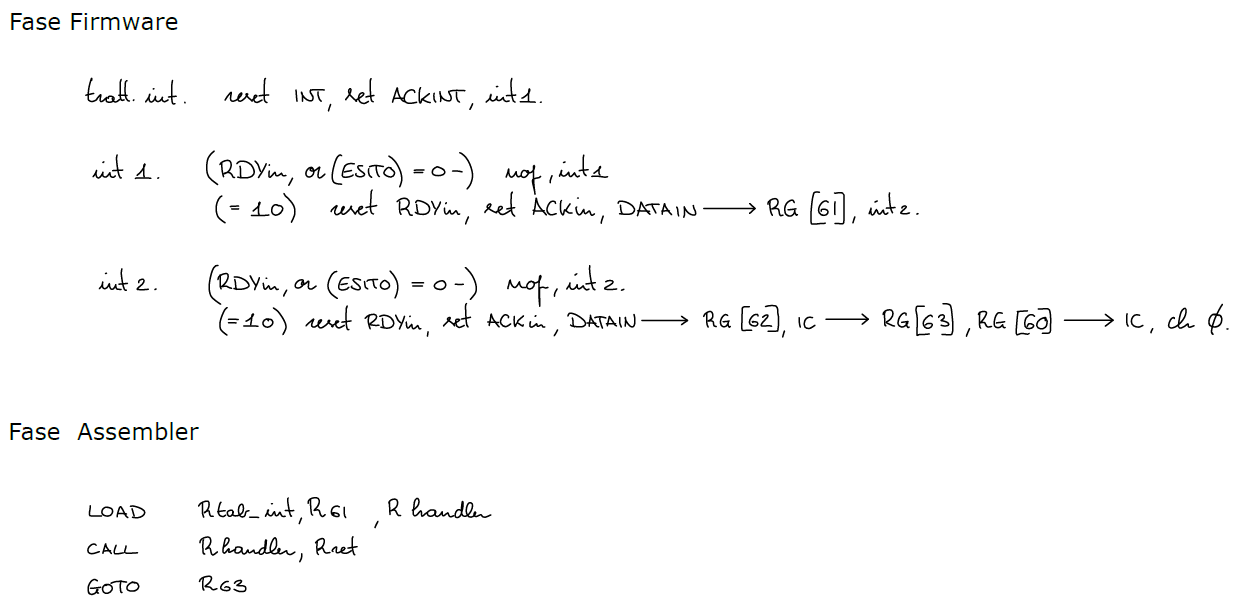
\includegraphics[width=\textwidth]{immagini/Handler.png}
\end{figure}
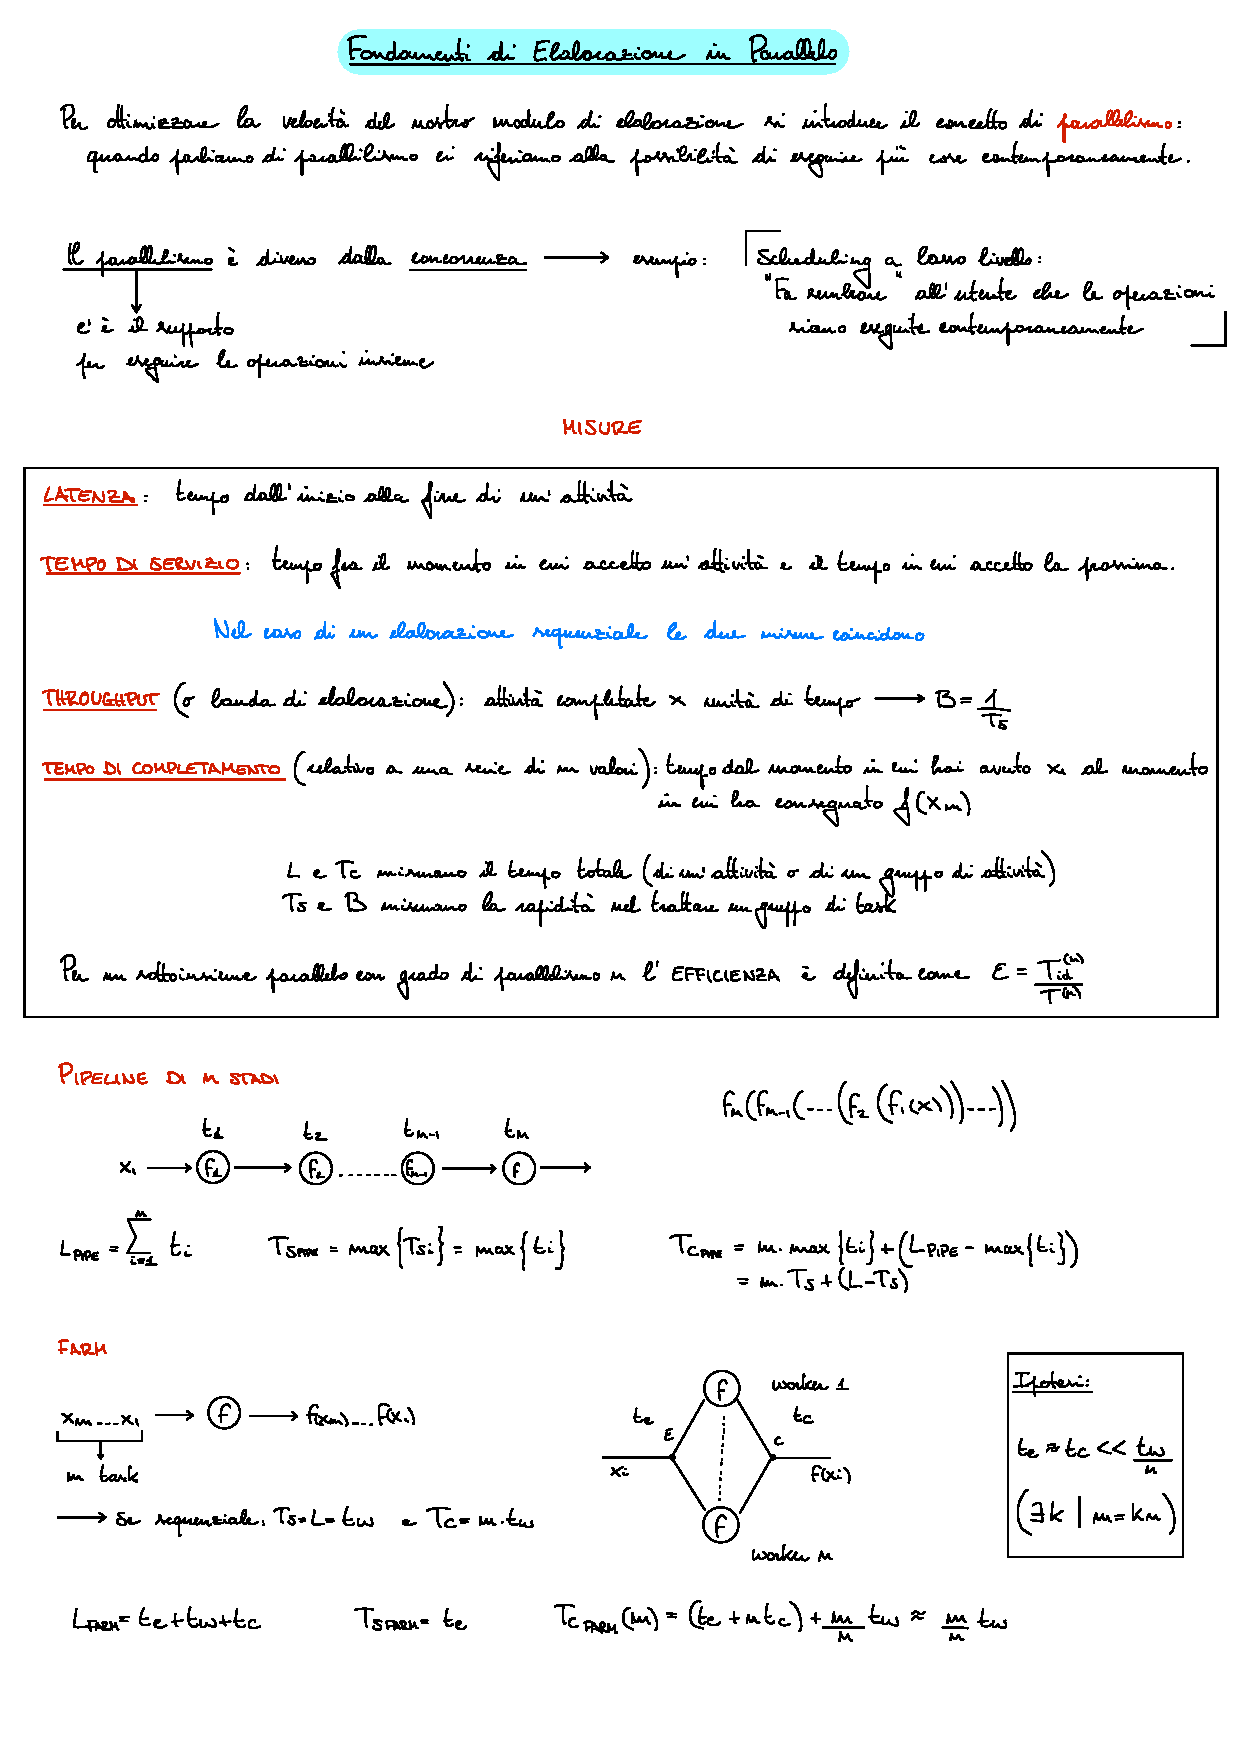
\includepdf[pages=-]{Elaborazione_parallelo}

